\documentclass[11pt,ngerman,a4paper]{article}
%Gummi|061|=)
\usepackage{amsmath}
\usepackage{a4wide}
\usepackage{amsthm}
\usepackage{amsbsy}
\usepackage{amssymb}
\usepackage{inputenc}
\usepackage{rotating} 
\usepackage{graphicx}
\usepackage{paralist}
\usepackage{selinput}
\SelectInputMappings{%
adieresis={ä},
germandbls={ß},
}
\title{\textbf{Versuch V355: Gekoppelte Schwingkreise}}
\author{Martin Bieker\\
		Julian Surmann\\
		\\
		Durchgef\"{u}hrt am 09.01.2014\\
		Tu Dortmund}
\date{}
\usepackage{graphicx}
\begin{document}
\renewcommand\tablename{Tabelle}
\renewcommand\figurename{Abbildung}
\maketitle
\thispagestyle{empty}
\newpage
\clearpage
\setcounter{page}{1}


\section{Einleitung}
Der folgende Versuch gekoppelte Oszillatoren untersucht werden. Bei diesen Systemen handelt es sich um schwingfähige Systeme, welche miteinander in Welchselwirkung stehen und so Energie austauschen können. 

\section{Theorie}

In diesem Versuch sollen zwei Schwingkreise untersucht werden, die über eine gemeinsame Koppelkapazität $C_K$ miteinander wechselwirken (siehe Abb \ref{theorie}). Mit Hilfe der Kirchhoffschen Gesetze kann gezeigt werden, dass der Verlauf der Ströme $I_1$ und $I_2$ durch zwei gekoppelte Differentialgleichungen zweiter Ordnung bestimmt wird. Daraus folgt, dass die $I_1$ und $I_2$ durch eine Überlagerung von zwei so genannten Fundamentalschwingungen beschreiben werden können. Diese haben die Frequenzen


\begin{equation}
\nu^+ = \frac{1}{2 \pi \sqrt{LC}}
\label{nueplus}
\end{equation}
und 
\begin{equation}
\nu^- =\frac1{2\pi\sqrt{L(\frac1C + \frac2{C_K})^-1}}.
\label{nueminus}
\end{equation}

\noindent
Im Folgenden soll der Stromverlauf für die Anfangesbedingungen
\[
I_1(0) = I_0 \neq 0
\] 
und 
\[
I_2(0) = 0
\]
untersucht werden. Zusätzlich wird angenommen, dass sich die Frequenzen $\nu_+$  und $\nu_-$ sich nur geringfügig unterscheiden. Den in diesem Fall auftretenden Schwingungsvorgang bezeichnet man als Schwebung. Dabei schwingen die Einzelkreise ungefähr mit der Frequenz $\nu_+$. Des weiteren ändert sich die Amplitude der Schwingung mit der Wesentlich geringeren Frequenz 
\begin{equation}
\nu_{Schwebung} = \nu_- - \nu_+
\end{equation}

\section{Aufbau und Durchf\"{u}hrung}
\subsection{Vorbereitungen}
Vor Beginn der Messungen müssen die Resoanzfrequnezen beider Schwinkreise aufeinander abgestimmt werden. Dazu wird die Schaltung wie in abbildung \ref{abb1} gezeigt aufgebaut.
\begin{figure}[htp]
\centering
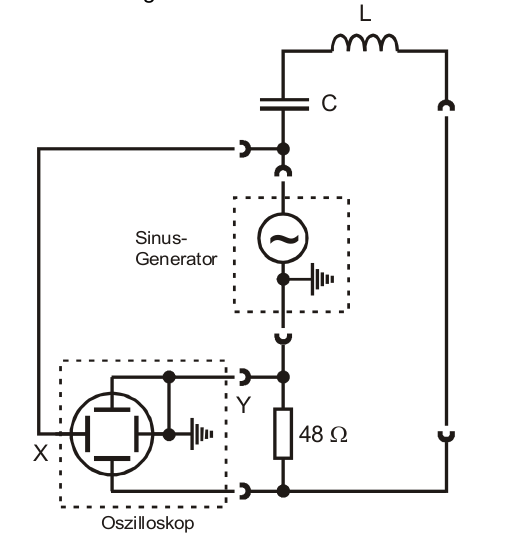
\includegraphics[scale=0.5]{Abb/abb1.png}
\caption{Schaltung zur Kalibrierung der Schwingkriese}
\label{abb1}
\end{figure}
In einem der Kreise ein Kondensator mit variabler Kapazität verbaut. Mit dem Sinusgenerator wird nun der Kreis mit konstanter Kapazi\"at angeregt. Zunächst wird mit dem Oszilloskop im YT-Betrieb die Frequenz ermittelt bei der die gemessene Spannung $U_R$ maximal wird. Dann wird das Oszilloskop in den XY-Modus umgeschaltet die Resonanzfrequnz $\nu_{res}$ bestimmt. Diese zeichnet sich dadurch aus, dass $U_R$ und die Generatorspannung $U_0$ in Phase liegen und daher die angezeigte Lissajouz-Figur eine Gerade ist. Danach wird der Sinusgenerator an den zweiten Teil des Schwingkreises angeschlossen und mit der Frequenz $\nu_{res}$ angeregt. Nun wird auch dieser Kreis durch Verändern der variablen Kapazität in Resonanz gebracht. Dazu werden wie zuvor Lissajouz-figuren verwendet. 
\subsection{Messung vom Schwebungs- und Schwingungsfrquenz}
Für diesen Versuchsteil wird die Schaltung wie in Abbildung \ref{abb2} aufgebaut.
\begin{figure}[h!]
\centering
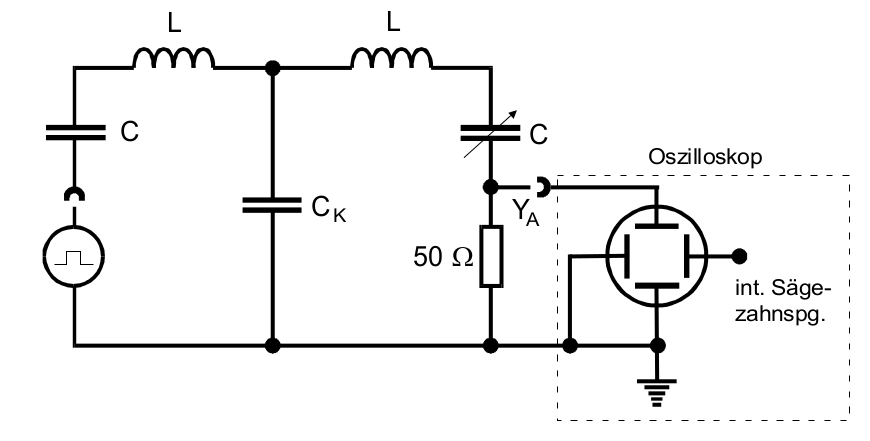
\includegraphics[scale=0.5]{Abb/abb2.png}
\caption{Schaltung zur Messung des Verhältnisses von Schwebungs- zu Schwingungfrequenz }
\label{abb2}
\end{figure}
 Der linke Schwingkreis wird durch eine Rechteckspannung zu Schwingungen angeregt. Mit dem Oszilloskop wird nun die am Widerstand $R$ abfallende Spannung gemessen. So kann der im rechten Schwingkreis fließende Strom bestimmt. Bei verschieden Koppelkapazitäten $C_K$ wird nun das Verhältnis von Schwingungs- und Schwebungsfrequenz bestimmt. Dazu wird die Zahl $n$ der Schwingungsmaxima in einer Schwebungsperiode bestimmt. Es gilt:
\begin{equation}
\frac{\nu_{Schwingung}}{\nu_{Schwebung}} = n
\end{equation}
\subsection{Messung der Frequenzen der Fundamentalschwingungen}
Des Weiteren sollen die Frequenzen $\nu_-$ und $\nu_+$ bestimmt werden. Diese zeichen sich dadurch aus, dass die Phasenverschiebung zwischen der Errgerspannung und dem im Sekundärkreis fließenden Stroms $0$ oder $\pi$ beträgt. Die oben Verwendete Schaltung wird nun mit einer Sinusspannung angeregt und die Generator auf den zweiten Kanal des Oszilloskops gelegt (siehe Abb. \ref{abb3}).
\begin{figure}[h!]
\centering
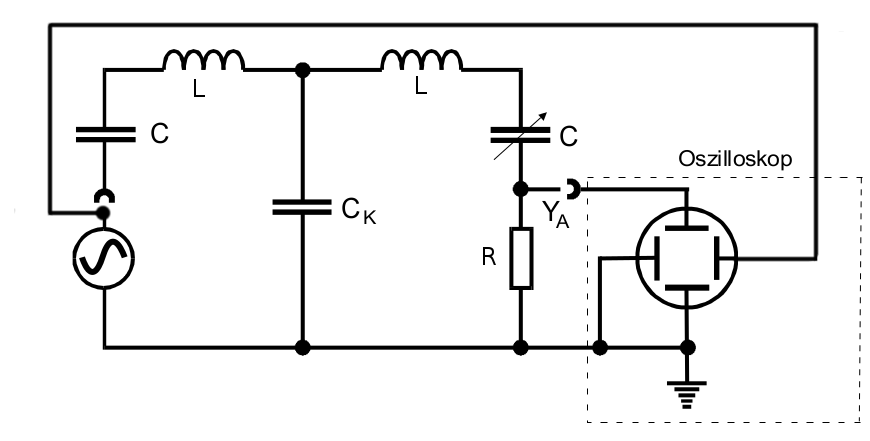
\includegraphics[scale=0.5]{Abb/abb3.png}
\caption{Schaltung zur Messung der Frequenzen der Fundamentalschwingungen}
\label{abb3}
\end{figure}
 So kann die Phasenbeziehung von $I$ und $U_0$ mit Hilfe von Lissajouz-Figuren untersucht werden. So werden $\nu_+$ und $\nu_-$ in Abhängikeit von $C_K$ bestimmt.
\subsection{Messung des Stroms in Abhängigkeit von der Erregerfrequenz}
Um den Verlauf des Stroms $I$ im Sekundärkreis bei in Abhängigkeit von der Erregerfrequenz darzustellen, wird die Schaltung wie in Abbildung \ref{abb1} aufgebaut. Mit dem Unterschied, dass der Funktionsgenerator im Sweep-Betreib arbeitet. Dies bedeutet, dass die Frequenz der Errgerspannung nicht mehr konstant ist, sondern steigt in der Zeit $\Delta t = ...\,s$ von $\nu_0 = ..\,Hz$ auf $\nu_1 = ..\,Hz$. Mit der Verlauf der am Widertsand abfallenden spannung gemessen werden. Dabei wird die Zeitbasis des Oszilloskops so eingestellt, dass ein vollständiger Sweep auf dem Schirm zu sehen ist. Anfang und Ende dieses Zyklus entsprechen den Frequenzen $\nu_0$ und $\nu_1$.     



\section{Auswertung}


Sofern nicht anders angegeben, wurden alle Fehler mit python uncertainties berechnet.
\subsection{Vorbereitungen}
Für die Justierung des Messaufbaus wurde mit der Grobmessung eine Frequenz von $(30.69\pm0.01)\,kHz$ ermittelt. Die feine Messung mit Hilfe der Lissajous-Figuren ergab eine Resonanzfrequenz von $(30.70\pm0.01) \, kHz$. Der mit L und C theoretisch berechnete Wert liegt bei $30.49 \, kHz$, mit einer Abweichung von $0.68 \%$ ausgezeichnet im Toleranzbereich. Allerdings wurde in der Berechnung des theoretischen Wertes die Kapazität der Spule schon berücksichtigt.
\subsection{Messung von Schwebungs- und Schwingungsfrequenz}
Die Perioden pro Schwebungsperiode wurden so genau wie möglich abgelesen. Der Fehler liegt bei maximal $\pm 0.5$ Perioden. Alle Werte sind der Tabelle \ref{AufgabeA} zu entnehmen.

\begin{table}[h]
\hspace{-2.6cm}
\begin{tabular}{|c|c|c|c|c|c|c|}
\hline
$C_K / 10^{-9}F$ & Freq.-Verhältnis & $\nu_{theo}^-/10kHz$ & $\overline{\nu_{theo}}/10kHz$ & $f_{Schwebung}/kHz$ & Freq-$V._{theo}$ & Abweichung/\% \\
\hline
$(2.03\pm0.06)$& $(3.5\pm0.5)$ & $(4.014\pm0.025)$& $(3.532\pm0.013)$& $(9.65\pm0.25)$& $(3.66\pm0.08)$ & $(4\pm14)$\\
$(3.00\pm0.09)$& $(4.5\pm0.5)$ & $(3.736\pm0.019)$& $(3.393\pm0.010)$& $(6.87\pm0.18)$& $(4.94\pm0.12)$ & $(9\pm10)$\\
$(4.00\pm0.12)$& $(6.5\pm0.5)$ & $(3.580\pm0.015)$& $(3.314\pm0.008)$& $(5.30\pm0.14)$& $(6.25\pm0.16)$ & $(4\pm8)$\\
$(5.02\pm0.15)$& $(8.0\pm0.5)$ & $(3.480\pm0.012)$& $(3.265\pm0.007)$& $(4.31\pm0.12)$& $(7.58\pm0.20)$ & $(6\pm7)$\\
$(6.47\pm0.19)$& $(9.8\pm0.5)$ & $(3.389\pm0.010)$& $(3.219\pm0.005)$& $(3.40\pm0.10)$& $(9.47\pm0.25)$ & $(3\pm6)$\\
$(8.00\pm0.24)$& $(11.0\pm0.5)$ & $(3.327\pm0.008)$& $(3.188\pm0.005)$& $(2.78\pm0.08)$& $(11.46\pm0.31)$ & $(4\pm5)$\\
$(9.99\pm0.30)$& $(13.0\pm0.5)$ & $(3.274\pm0.007)$& $(3.162\pm0.004)$& $(2.25\pm0.06)$& $(14.1\pm0.4)$ & $(7\pm4)$\\
\hline
\end{tabular}
\caption{Untersuchung der Schwebungsvorgänge}
\label{AufgabeA}
\end{table}\noindent
$\nu_{theo}^+$ ist konstant und beträgt $(30493\pm25)\,Hz$. Er wurde mit Formel \ref{nueplus} berechnet. Der bei $C_K$ angegebene Fehler ist ein auf die Werte umgerechneter Fehler von $\pm 3 \%$. Dieser ist an der Messapparatur vorgegeben. $\nu_{theo}^-$ wurde mit Formel \ref{nueminus} ermittelt. Der Mittelwert der beiden Frequenzen wurde mit $\overline{X}=\frac{1}{2}(X_a+X_b)$ ermittelt. Die Frequenz der Schwebung ist durch $\nu_{theo}^--\nu_{theo}^+$ gegeben. Die Abweichung in \% zeigt die Abweichung vom experimentellen zum theoretischen Frequenzverhältnis. Da die Ermittlung des experimentellen Verhältnisses mit $\pm0.5$ recht ungenau war, sind die Abweichungen vom sehr genauen Theoriewert in Ordnung.
\subsection{Messung der Frequenzen der Fundamentalschwingungen}
Für die Messung der Frequenzen wurden Lissajous-Figuren benutzt. Die Frequenzen des Signalgenerators wurden bei bestehen einer Geraden aufgenommen. Die Frequenzen werden in Tabelle \ref{AufgabeB} mit den Theoriewerten aus 4.2 Verglichen.
\begin{table}[h] 
\hspace{-1.9cm}
\begin{tabular}{|c|c|c|c|c|c|c|}
\hline
$C_K / 10^{-9}F$ & $\nu_{theo}^+/10kHz$ & $\nu_{theo}^-/10kHz$ & $\nu_{exp}^+/Hz$ & $\nu_{exp}^-/Hz$ & Abweichung $\nu^+/\%$ & Abweichung $\nu^-/\%$ \\
\hline
$(2.03\pm0.06)$ & $(30493\pm25)$ & $(4.014\pm0.025)$ & 30490 & 40010 & $(0.9999\pm0.0008)$ & $(0.997\pm0.006)$\\
$(3.00\pm0.09)$& $(30493\pm25)$ & $(3.736\pm0.019)$ & 30490 & 37300 & $(0.9999\pm0.0008)$ & $(0.998\pm0.005)$\\
$(4.00\pm0.12)$& $(30493\pm25)$ & $(3.580\pm0.015)$ & 30490 & 35760 & $(0.9999\pm0.0008)$ & $(0.999\pm0.004)$\\
$(5.02\pm0.15)$& $(30493\pm25)$ & $(3.480\pm0.012)$ & 30490 & 34780 & $(0.9999\pm0.0008)$ & $(0.9995\pm0.0035)$\\
$(6.47\pm0.19)$& $(30493\pm25)$ & $(3.389\pm0.010)$ & 30490 & 33880 & $(0.9999\pm0.0008)$ & $(0.9997\pm0.0029)$\\
$(8.00\pm0.24)$& $(30493\pm25)$ & $(3.327\pm0.008)$ & 30490 & 33280 & $(0.9999\pm0.0008)$ & $(1.0002\pm0.0025)$\\
$(9.99\pm0.30)$& $(30493\pm25)$ & $(3.274\pm0.007)$ & 30490 & 33750 & $(0.9999\pm0.0008)$ & $(1.0308\pm0.0022)$\\
\hline
\end{tabular}
\caption{Frequenzen der Fundamentalschwingung}
\label{AufgabeB}
\end{table}
Die Berechnung zeigt eine Abweichung vom Theoriewert von jeweils ca. 1 \%.
\subsection{Messung des Stroms in Abhängigkeit von der Erregerfrequenz}
Die in dieser Messreihe aufgenommenen Werte sind in Tabelle \ref{AufgabeC} ersichlich.
\begin{table}[h] 
\begin{tabular}{|c|c|c|c|c|c|}
\hline
$C_K \,/ 10^{-9}F$ & Zeit / ms & $d_1\,/ms$ & $d_2\,/ms$ & Peak $U_1\,/V$ & Peak $U_1\,/V$ \\
\hline
$(1.01\pm0.03)$ & 21 & $(9\pm0.5)$ & $(13.7\pm0.5)$ & $(1.22\pm0.05)$ & $(0.90\pm0.05)$ \\
$(2.03\pm0.06)$ & 21 & $(9\pm0.5)$ & $(11.8\pm0.5)$ & $(1.25\pm0.05)$ & $(1.02\pm0.05)$ \\
$(3.00\pm0.09)$& 21 & $(9\pm0.5)$ & $(10.9\pm0.5)$ & $(1.25\pm0.05)$ & $(1.10\pm0.05)$ \\
$(4.00\pm0.12)$& 21 & $(9\pm0.5)$ & $(10.5\pm0.5)$ & $(1.30\pm0.05)$ & $(1.15\pm0.05)$ \\
$(5.02\pm0.15)$& 21 & $(9\pm0.5)$ & $(10.1\pm0.5)$ & $(1.33\pm0.05)$ & $(1.19\pm0.05)$ \\
$(6.47\pm0.19)$& 21 & $(9\pm0.5)$ & $(9.9\pm0.5)$ & $(1.40\pm0.05)$ & $(1.30\pm0.05)$ \\
$(8.00\pm0.24)$& 21 & $(9\pm0.5)$ & $(9.5\pm0.5)$ & $(1.46\pm0.05)$ & $(1.34\pm0.05)$ \\
$(9.99\pm0.30)$& 21 & $(9\pm0.5)$ & $(9.5\pm0.5)$ & $(1.55\pm0.05)$ & $(1.43\pm0.05)$ \\
\hline
\end{tabular}
\caption{Messdaten des dritten Versuchsteils}
\label{AufgabeC}
\end{table}
Die bei den zeitlichen Abständen und der Spannung angegebenen Unsicherheiten entsprechen der Hälfte der kleinsten angezeigten Skaleneinteilungen des Oszilloskops. Aus den zeitlichen Abständen $d_1$ und $d_2$ kann mit folgenden Zusammenhängen die zugehörige Frequenz berechnet werden:
\begin{itemize}
\item $f_1 = \frac{70400\cdot d_1}{21}+3800$
\item $f_2 = \frac{70400\cdot d_2}{21}+3800$.
\end{itemize}
Die Frequenzen sind in Tabelle \ref{AufgabeC2} angegeben. Die Ströme wurden mit dem Ohmschen Gesetz berechnet. Allerdings wurde der Widerstand mit 73 $\Omega$ statt mit 48 $\Omega$ angenommen, da weitere Dämpfungseffekte auftreten.
\begin{table}[h] 
\begin{tabular}{|c|c|c|c|c|}
\hline
$C_K \,/ 10^{-9}F$  & $f_1\,/10\, kHz$ & $f_2\,/10\,kHz$ & $I_1\,/A$ & $I_1\,/A$ \\
\hline
$(1.01\pm0.03)$  & $(3.40\pm0.17)$ & $(4.97\pm0.17)$ & $(0.0167\pm0.0007)$ & $(0.0123\pm0.0007)$ \\
$(2.03\pm0.06)$ & $(3.40\pm0.17)$ & $(4.34\pm0.17)$ & $(0.0171\pm0.0007)$ & $(0.0140\pm0.0007)$ \\
$(3.00\pm0.09)$ & $(3.40\pm0.17)$ & $(4.03\pm0.17)$ & $(0.0171\pm0.0007)$ & $(0.0151\pm0.0007)$ \\
$(4.00\pm0.12)$ & $(3.40\pm0.17)$ & $(3.77\pm0.17)$ & $(0.0178\pm0.0007)$ & $(0.0158\pm0.0007)$ \\
$(5.02\pm0.15)$& $(3.40\pm0.17)$ & $(3.70\pm0.17)$ & $(0.0182\pm0.0007)$ & $(0.0163\pm0.0007)$ \\
$(6.47\pm0.19)$& $(3.40\pm0.17)$ & $(3.56\pm0.17)$ & $(0.0192\pm0.0007)$ & $(0.0178\pm0.0007)$ \\
$(8.00\pm0.24)$ & $(3.40\pm0.17)$ & $(3.56\pm0.17)$ & $(0.0200\pm0.0007)$ & $(0.0184\pm0.0007)$ \\
$(9.99\pm0.30)$ & $(3.40\pm0.17)$ & $(9.5\pm0.17)$ & $(0.0212\pm0.0007)$ & $(0.0196\pm0.0007)$ \\
\hline
\end{tabular}
\caption{Auswertung des dritten Versuchsteils}
\label{AufgabeC2}
\end{table}
\section{Diskussion}
Insgesamt sind alle Unsicherheiten innerhalb der üblichen Toleranzen. Die Messfehler beim Ablesen der Werte auf dem Bildschirm des Oszilloskopes wurden eher pessimistisch angenommen, sie sind auf jeden Fall groß genug angenommen. Die Abweichungen der experimentellen zu den theoretischen Frequenzen sind mit $<$ 10 \% tolerierbar.\newline
In den anderen Versuchsteilen sind die Abweichungen alle gering.
\section{Abbildungsverzeichnis}
\begin{itemize}
\item Abb. 1: entnommen aus [1]
\item Abb. 2 und 3: entnommen aus [1] und geringfügig bearbeitet 
\end{itemize}
\section{Quellen}
\begin{enumerate}[{[}1{]}]
\item Anleitung: \textit{Versuch Nr.355 Gekoppelte Schwingkreise}, TU Dortmund 
\end{enumerate}
\section{Anhang}
\begin{itemize}
\item Tabellen
\item Auszug aus dem Messheft


\end{itemize}

\newpage
\end{document}v